% ============================================================
% Body sections for the Wearables paper
% ============================================================

\section{Introduction}\label{sec:intro}

\subsection{The wearable underwriting moment}\label{ss:moment}

By the end of 2025, the installed base of consumer wearables capable
of continuous biometric telemetry had exceeded 300 million devices.
Apple Watch, Fitbit (Google), Garmin, Oura, and Whoop together account
for the majority of this volume, with rapid market share gains by
ring-form-factor devices (Oura, Ultrahuman, RingConn) that prioritise
nightly metrics over fitness tracking. Within the actuarial sphere,
four large life insurers have moved from pilot programmes to mainstream
integration: John Hancock Vitality \citep{Hancock2018}, Manulife Move,
Discovery Vitality (South Africa, since 2010 the global pioneer), and
Prudential PRUActive. Several smaller insurers, including YuLife and
the digital-first carrier Ladder Life, integrate wearable signals
directly into pricing rather than as a loyalty wrapper.

The legacy life-underwriting workflow---paramedical examination,
attending-physician statements, MIB and Rx database checks, and the
underwriter's adjudication---is a slow, expensive, point-in-time
estimator of mortality risk. The wearable workflow is a fast,
continuous, longitudinal estimator. Both produce information about the
same latent quantity: the policyholder's all-cause mortality intensity
$\lambda_x(t)$. The actuarial profession's task is to combine the two
information sources, weight them by their relative credibility, and
preserve the contractual and regulatory protections that make life
insurance a socially trusted instrument.

\subsection{Why traditional credibility theory needs extension}\label{ss:why-credibility}

Classical credibility theory \citep{Buhlmann1967,BuhlmannGisler2005}
provides the standard machinery for blending a prior estimate with
observed experience: the credibility-weighted estimator
\begin{equation}\label{eq:classical-cred}
   \hat\mu_{\mathrm{cred}} \;=\; Z\,\hat\mu_{\mathrm{obs}}
   \;+\; (1-Z)\,\mu_{\mathrm{prior}},
\end{equation}
with the credibility weight $Z\in[0,1]$ a function of the precision of
the observation relative to the prior. Three features of the wearable
problem strain~\eqref{eq:classical-cred}:

\begin{enumerate}[leftmargin=*,nosep,topsep=4pt]
   \item \textbf{The observation is multidimensional and continuous.}
         A B\"uhlmann update treats $\hat\mu_{\mathrm{obs}}$ as a single
         summary statistic of a discrete-time experience window.
         Wearable telemetry is a vector-valued continuous-time process
         whose components have very different signal-to-noise ratios.
   \item \textbf{The prior is itself updated by wearable signals
         \emph{before} mortality experience accrues.} The applicant's
         twelve-month history of resting HR is a prior input to
         underwriting; subsequent telemetry is then a posterior update.
         The two roles must be distinguished cleanly or double-counting
         results.
   \item \textbf{Selection on observability.} Wearable owners are
         systematically wealthier, healthier, more digitally engaged,
         and on average younger than the general insured population.
         A na\"ive credibility weight estimated on a wearable-only
         sample over-states the precision of the signal for the
         broader pool.
\end{enumerate}

Sections~\ref{sec:taxonomy}--\ref{sec:credibility} address (1) and (2);
\S\ref{sec:selection} addresses (3).

\subsection{Our contribution}\label{ss:contrib}

We propose an integrated framework that:

\begin{enumerate}[leftmargin=*,nosep,topsep=4pt]
   \item Specifies the wearable signal taxonomy with an explicit
         actuarial-informativeness ranking
         (\S\ref{sec:taxonomy}, Table~\ref{tab:signals}).
   \item Formalises the Holmstr\"om informativeness principle for the
         wearable-augmented underwriting contract
         (\S\ref{sec:holmstrom}, Proposition~\ref{prop:holmstrom}).
   \item Derives the Bayesian credibility update for a multi-signal
         Poisson-Gamma mortality intensity, with closed-form
         credibility weight $Z(t)$ and asymptotic convergence rate
         (\S\ref{sec:credibility}, eqs.~\eqref{eq:posterior}--\eqref{eq:Z}).
   \item Maps the posterior intensity to an exponential-tilt premium
         adjustment with closed-form sensitivity
         (\S\ref{sec:premium}, eq.~\eqref{eq:premium-tilt}).
   \item Analyses the three failure modes (selection,
         substitution, intergenerational fairness) with concrete
         mitigations (\S\S\ref{sec:selection}--\ref{sec:fairness}).
   \item Compares the admissibility regimes under POPIA, GDPR, HIPAA,
         and the NY DFS Circular Letter 2019-1
         (\S\ref{sec:regulatory}, Table~\ref{tab:regulatory}).
   \item Works through a numerical example pricing a 25-year-old
         applicant with twelve months of Apple Watch telemetry
         (\S\ref{sec:worked}).
\end{enumerate}

The framework is presented in the same series as the earlier paper on
hyperscale data-center insurance \citep{Denewade2026DC}: the central
actuarial state variables are the mortality intensity $\lambda(t)$,
the credibility weight $Z(t)$, the premium $P^{\mathrm{tech}}$, and
the underwriting-class indicator $\mathcal{U}\in\{\mathrm{Std},
\mathrm{Pref},\mathrm{Pref+}\}$. Every wearable quantity introduced
in the body routes back to one of these.

% ============================================================
\section{The wearable biometric signal taxonomy}\label{sec:taxonomy}

\subsection{What wearables actually measure}\label{ss:measure}

Consumer wearables sense a small number of underlying physical
quantities and derive a larger number of summary metrics from them
through proprietary algorithms. The base sensors are:

\begin{itemize}[leftmargin=*,nosep,topsep=4pt]
   \item \textbf{Photoplethysmography (PPG)} ---
         optical heart rate via reflected green/red/IR light. Sampling
         rate $25$--$\SI{100}{\hertz}$. From PPG the device derives
         resting HR, HR during activity, HR recovery, and (with
         spectral processing) heart-rate variability metrics.
   \item \textbf{Electrocardiography (ECG)} ---
         single-lead ECG (Apple Watch Series 4+; Fitbit Sense; Galaxy
         Watch). Used for AFib screening and high-fidelity HRV.
   \item \textbf{Pulse oximetry (SpO$_2$)} ---
         red/IR PPG ratio. Estimates blood oxygen saturation, mainly
         used for nightly minima and altitude alerts.
   \item \textbf{Inertial measurement (IMU)} ---
         3-axis accelerometer plus gyroscope. Drives step counts,
         activity recognition, fall detection, and (combined with PPG)
         sleep-stage classification.
   \item \textbf{Skin temperature} ---
         contact thermistor, $\SI{1}{\milli\kelvin}$ resolution.
         Recent devices (Apple Watch Series 8+, Oura Ring) track
         nightly skin-temperature deviation from the personal
         baseline.
\end{itemize}

\begin{figure}[ht]
\centering
\begin{tikzpicture}[
   every node/.style={font=\footnotesize},
   sensor/.style={draw,rounded corners=2pt,fill=blue!8,
                  minimum width=2.0cm,minimum height=0.55cm,align=center},
   derived/.style={draw,rounded corners=2pt,fill=orange!10,
                   minimum width=2.0cm,minimum height=0.55cm,align=center},
   actuarial/.style={draw,rounded corners=2pt,fill=red!10,
                     minimum width=2.4cm,minimum height=0.6cm,align=center,
                     font=\footnotesize\bfseries},
   arr/.style={->,thick,gray!70!black,-{Latex[length=2mm]}},
   label/.style={font=\scriptsize,gray}
]

% Sensors (left column)
\node[sensor] (PPG) at (0,3.5) {PPG};
\node[sensor] (ECG) at (0,2.5) {ECG};
\node[sensor] (SPO) at (0,1.5) {SpO$_2$};
\node[sensor] (IMU) at (0,0.5) {IMU};
\node[sensor] (TEMP) at (0,-0.5) {Skin temp};

% Derived metrics (middle column)
\node[derived] (RHR) at (4.8,4.0) {Resting HR};
\node[derived] (HRV) at (4.8,3.0) {HRV (RMSSD)};
\node[derived] (HRREC) at (4.8,2.0) {HR recovery};
\node[derived] (SPO2N) at (4.8,1.0) {SpO$_2$ nadir};
\node[derived] (STEPS) at (4.8,0.0) {Step distribution};
\node[derived] (SLEEP) at (4.8,-1.0) {Sleep efficiency};
\node[derived] (TEMPDEV) at (4.8,-2.0) {Temp deviation};

% Actuarial variables (right column)
\node[actuarial] (LAMBDA) at (10.0,2.5) {$\lambda(t)$};
\node[actuarial] (Z) at (10.0,1.0) {$Z(t)$};
\node[actuarial] (P) at (10.0,-0.5) {$P^{\mathrm{tech}}$};

% Sensor -> Derived arrows
\draw[arr] (PPG.east) -- (RHR.west);
\draw[arr] (PPG.east) -- (HRV.west);
\draw[arr] (PPG.east) -- (HRREC.west);
\draw[arr] (ECG.east) -- (HRV.west);
\draw[arr] (SPO.east) -- (SPO2N.west);
\draw[arr] (IMU.east) -- (STEPS.west);
\draw[arr] (IMU.east) -- (SLEEP.west);
\draw[arr] (PPG.east) -- (SLEEP.west);
\draw[arr] (TEMP.east) -- (TEMPDEV.west);

% Derived -> actuarial arrows (showing the informativeness flow)
\draw[arr,iaaccent] (RHR.east) -- (LAMBDA.west);
\draw[arr,iaaccent] (HRV.east) -- (LAMBDA.west);
\draw[arr,iaaccent] (HRREC.east) -- (LAMBDA.west);
\draw[arr,iaaccent] (SPO2N.east) -- (LAMBDA.west);
\draw[arr,iaaccent] (STEPS.east) -- (LAMBDA.west);
\draw[arr,iaaccent] (SLEEP.east) -- (LAMBDA.west);
\draw[arr,iaaccent] (TEMPDEV.east) -- (LAMBDA.west);

% Actuarial cascade
\draw[arr,iadark,line width=0.8pt] (LAMBDA.south) -- (Z.north);
\draw[arr,iadark,line width=0.8pt] (Z.south) -- (P.north);

% Column labels
\node[label,font=\scriptsize\bfseries] at (0,4.6) {Physical sensors};
\node[label,font=\scriptsize\bfseries] at (4.8,4.8) {Derived metrics};
\node[label,font=\scriptsize\bfseries] at (10.0,3.5) {Actuarial state};

\end{tikzpicture}
\caption{The wearable signal flow from physical sensors (blue) through
derived metrics (orange) to actuarial state variables (red). Each
derived metric is a candidate input to the mortality intensity
$\lambda(t)$; the credibility weight $Z(t)$ controls how much the
posterior moves toward the wearable evidence; the premium
$P^{\mathrm{tech}}$ is a deterministic function of the posterior.}
\label{fig:signal-flow}
\end{figure}

\subsection{Informativeness ranking}\label{ss:rank}

The starting point for our framework is an empirical ranking of
wearable-derived metrics by their incremental information content
with respect to all-cause mortality, adjusted for age and sex. The
ranking is itself an actuarial output of analyses on the UK Biobank
\citep{Biobank2024}, the All of Us research programme, and the
proprietary cohorts of Discovery Vitality and John Hancock Vitality
where published meta-analyses are available.

\begin{table}[ht]
\centering\small
\caption{Wearable-derived metrics ranked by approximate incremental
information content for all-cause mortality, conditional on age, sex
and BMI. Hazard ratios are illustrative; binding values depend on the
specific cohort and follow-up window. ``Tier'' is the recommended
underwriting weight class. Source synthesis from
\cite{Strain2020,Hippisley2017,Biobank2024} and proprietary
disclosures.}\label{tab:signals}
\setlength{\tabcolsep}{5pt}
\begin{tabular}{p{3.6cm}cccc}
\toprule
Metric & Typical HR (top vs bottom decile) & Confounding & Gameability & Tier \\
\midrule
Resting HR (12-mo median)        & 1.6--2.0 & age, fitness           & low    & A \\
Sleep efficiency (12-mo median)  & 1.3--1.6 & shift work, alcohol   & medium & B \\
HRV (RMSSD, 12-mo median)        & 1.4--1.8 & stress, training load & medium & B \\
SpO$_2$ nadir (nightly)          & 1.5--2.2 & altitude, sleep apnea & low    & A \\
Step count (12-mo median)        & 1.4--1.9 & device-not-worn bias  & high   & C \\
HR recovery 1\,min post-exercise & 1.6--2.5 & training adherence    & high   & C \\
Nightly temp deviation           & 1.2--1.4 & illness, hormonal     & low    & B \\
$\dot{V}\mathrm{O}_2$ max proxy  & 1.7--2.4 & altitude, illness    & low    & A \\
Atrial fibrillation alert        & 2.5--4.0 & age, cardiac history  & low    & A \\
\bottomrule
\end{tabular}
\end{table}

Tier A metrics --- resting HR, SpO$_2$ nadir, $\dot{V}\mathrm{O}_2$-max
proxy, AFib alerts --- are the foundation of any wearable underwriting
programme: high information content, low gameability, robust to
device-not-worn bias because they are nightly or per-session rather
than continuous-aggregated. Tier C metrics --- step counts, HR
recovery --- carry serious gameability concerns and should enter the
contract only at heavily discounted credibility weights or as part of
a verified-protocol challenge (e.g.\ a supervised 6-minute walk test
at policy issue).

\begin{rbox}
The signal-flow diagram of Figure~\ref{fig:signal-flow} embeds an
\emph{actuarial} hypothesis: each derived metric contributes to a
single scalar mortality intensity $\lambda(t)$. This is the natural
default but it is not the only choice. For impairment-specific covers
(critical illness, dread disease) one may wish to decompose
$\lambda(t)$ into cause-specific intensities $\lambda^{\mathrm{CV}}(t)$,
$\lambda^{\mathrm{CA}}(t)$, $\lambda^{\mathrm{other}}(t)$ and route the
SpO$_2$ signal preferentially into the cardiovascular component. This
generalisation is a straightforward extension of the framework below.
\end{rbox}

% ============================================================
\section{The Holmstr\"om informativeness principle formalised}\label{sec:holmstrom}

The Holmstr\"om informativeness principle \citep{Holmstrom1979} is the
foundational result of principal--agent theory: in an optimal contract,
any additional signal that is statistically informative about the
agent's hidden action or type should enter the contract with non-zero
weight. In the underwriting context the ``agent'' is the applicant
(whose mortality type is hidden) and the ``signal'' is the wearable
telemetry.

\begin{proposition}[Wearable informativeness]\label{prop:holmstrom}
Let $\mathcal{U}\in\{\mathrm{Std},\mathrm{Pref},\mathrm{Pref+}\}$ be
the underwriting class assignment, $T$ the residual lifetime of the
applicant, and $\mathbf{W}=(W_1,\dots,W_k)$ the vector of wearable
metrics observed over a finite window $[0,\tau]$. If
$\mathbf{W}\not\perp T \mid \mathcal{U}$, then the underwriting
contract that ignores $\mathbf{W}$ is Pareto-dominated by a contract
that conditions the premium on $\mathbf{W}$.
\end{proposition}

\begin{proof}[Proof sketch] Standard Holmstr\"om-Mirrlees argument:
the conditional likelihood ratio
$f(T\mid\mathcal{U},\mathbf{W})/f(T\mid\mathcal{U})$ is non-degenerate
under the informativeness hypothesis, and the value function of the
insurer's pricing problem is strictly increasing in the information
content of the conditioning sigma-algebra
$\sigma(\mathcal{U},\mathbf{W}) \supsetneq \sigma(\mathcal{U})$.
The Lagrangian optimum therefore places a strictly positive weight on
$\mathbf{W}$. $\square$
\end{proof}

The proposition is the actuarial-economic justification for using
wearable signals. It does not, by itself, tell us \emph{how much}
weight to place on each signal --- that is the credibility-weight
problem of the next section.

\begin{nbox}
Proposition~\ref{prop:holmstrom} also provides the formal answer to
the question: ``Should wearable signals be mandatory or optional in
the policy contract?'' The Pareto-improvement is conditional on the
applicant agreeing to share the signal. A mandatory regime is
Pareto-dominant on actuarial grounds but Pareto-dominated by an
opt-in regime that respects autonomy. The optimal regime is therefore
opt-in with a transparent premium reduction for participants, which
is exactly the structure adopted by Vitality, John Hancock, and
Manulife. The framework of this paper supplies the pricing schedule
for the participation reduction.
\end{nbox}

% ============================================================
\section{Bayesian credibility for wearable-augmented mortality}\label{sec:credibility}

\subsection{The prior intensity}\label{ss:prior}

For an applicant of age $x$, sex $s$, and standard underwriting
covariates $\mathbf{z}$ (BMI, smoking status, family history, etc.),
the prior mortality intensity is the actuary's pre-wearable
benchmark:
\begin{equation}\label{eq:prior}
   \lambda_0(x,s,\mathbf{z}) \;=\;
   \mu^{\mathrm{base}}(x,s) \cdot \exp\!\bigl(\bm{\beta}^\top \mathbf{z}\bigr),
\end{equation}
with $\mu^{\mathrm{base}}(x,s)$ the period mortality from a published
table (e.g.\ SOA 2017 CSO for the US, A2010 for South Africa, ELT17
for the UK), and $\bm{\beta}^\top\mathbf{z}$ a Cox-style log-linear
adjustment from the insurer's experience studies. This is the
standard pre-wearable starting point.

\subsection{The wearable likelihood}\label{ss:lik}

Let $\mathbf{W}_t = (W_1(t),\dots,W_k(t))$ denote the wearable-metric
vector observed over a window of length $t$, and let
$\bar{\mathbf{W}}_t$ denote the windowed sample mean. We adopt a
log-linear specification for the conditional intensity:
\begin{equation}\label{eq:loglinear}
   \lambda(t \mid \bar{\mathbf{W}}_t)
   \;=\; \lambda_0(x,s,\mathbf{z}) \cdot
         \exp\!\Bigl(\sum_{j=1}^k \gamma_j \cdot
                     \tilde W_j(t)\Bigr),
\end{equation}
where $\tilde W_j(t)$ is the standardised metric (centred and scaled
by the age/sex-specific population distribution) and $\gamma_j$ is
the metric's mortality-elasticity coefficient. The coefficients
$\gamma_j$ are themselves the object of inference; we treat them as
deterministic, pre-fitted from the cohort studies of
Table~\ref{tab:signals}.

\subsection{The Poisson-Gamma credibility update}\label{ss:cred-update}

Following classical credibility theory, treat the latent applicant
intensity $\Lambda$ as Gamma-distributed with shape
$\alpha_0=\nu$ and rate $\beta_0=\nu/\lambda_0$ (so that $\E[\Lambda]
= \lambda_0$ and the prior precision is governed by $\nu$). Suppose
the wearable window $[0,t]$ yields observed counts of metric-derived
``mortality-equivalent events'' $N_t$ that, conditional on $\Lambda$,
are Poisson$(\Lambda\,t)$. Standard conjugacy gives the posterior:
\begin{equation}\label{eq:posterior}
   \Lambda \given N_t = n_t \;\sim\;
   \mathrm{Gamma}\!\bigl(\nu + n_t,\;
                          \nu/\lambda_0 + t\bigr),
\end{equation}
with posterior mean
\begin{equation}\label{eq:postmean}
   \E[\Lambda \given N_t = n_t]
   \;=\; \frac{\nu + n_t}{\nu/\lambda_0 + t}
   \;=\; Z(t)\cdot \frac{n_t}{t}
        + \bigl(1-Z(t)\bigr)\cdot \lambda_0,
\end{equation}
where the credibility weight is
\begin{equation}\label{eq:Z}
   \boxed{\;Z(t) \;=\; \frac{t}{t + \nu/\lambda_0}.\;}
\end{equation}
Equation~\eqref{eq:Z} is the central result of the credibility
section: the weight on wearable evidence is a hyperbolic function of
the observation window $t$, with the prior-precision parameter
$\nu/\lambda_0$ controlling how quickly the posterior moves toward
the evidence.

\begin{figure}[ht]
\centering
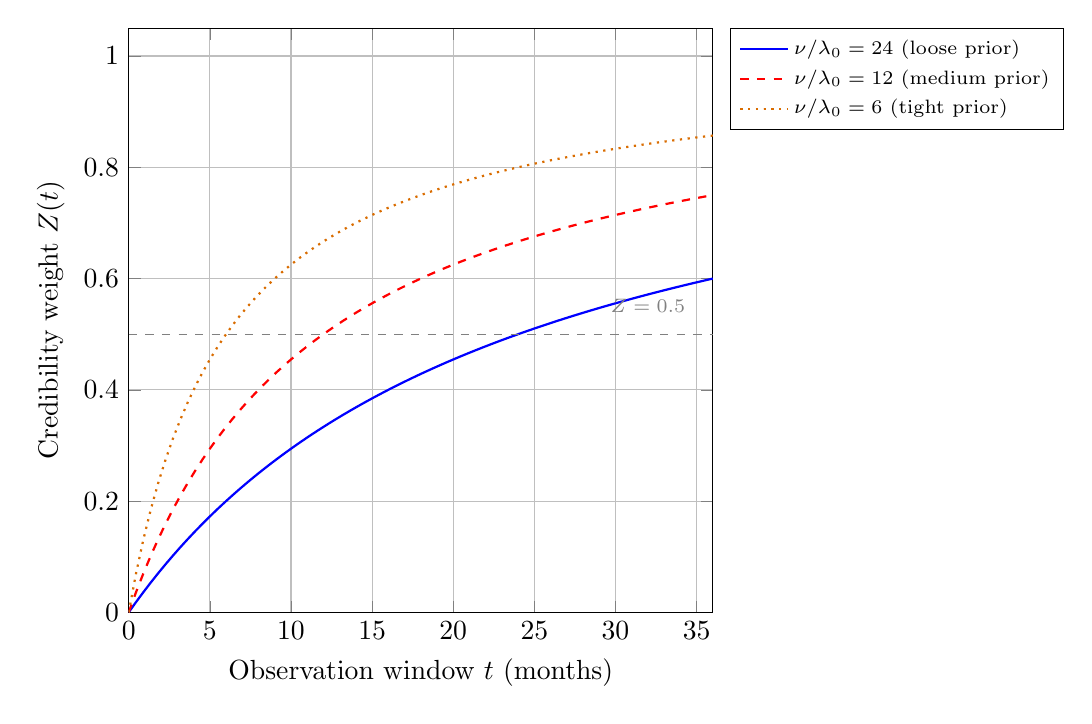
\begin{tikzpicture}
\begin{axis}[
   width=9cm, height=9cm,
   xlabel={Observation window $t$ (months)},
   ylabel={Credibility weight $Z(t)$},
   xmin=0, xmax=36, ymin=0, ymax=1.05,
   grid=major,
   legend pos=outer north east,
   legend cell align=left,
   legend style={font=\scriptsize}
]
% Three prior-precision regimes
\addplot[blue,thick,domain=0:36,samples=80]
   {x/(x+24)};
\addlegendentry{$\nu/\lambda_0 = 24$ (loose prior)}
\addplot[red,thick,dashed,domain=0:36,samples=80]
   {x/(x+12)};
\addlegendentry{$\nu/\lambda_0 = 12$ (medium prior)}
\addplot[orange!85!black,thick,dotted,domain=0:36,samples=80]
   {x/(x+6)};
\addlegendentry{$\nu/\lambda_0 = 6$ (tight prior)}
% Annotate Z=0.5 line
\draw[gray,dashed] (axis cs:0,0.5) -- (axis cs:36,0.5);
\node[gray,font=\scriptsize] at (axis cs:32,0.55) {$Z=0.5$};
\end{axis}
\end{tikzpicture}
\caption{Credibility weight $Z(t)$ from~\eqref{eq:Z} as a function of
the wearable observation window, for three prior-precision regimes.
A loose prior (much uncertainty about the applicant's true intensity)
moves the posterior toward the wearable evidence rapidly; a tight
prior holds the posterior near the table mortality longer. At
$Z(t)=0.5$ the posterior places equal weight on the wearable
evidence and the table prior --- the natural decision boundary for
``does this wearable history reclassify the applicant?''.}
\label{fig:Z-convergence}
\end{figure}

\subsection{Asymptotic behaviour}\label{ss:asymp}

As $t\to\infty$, $Z(t)\to 1$ and the posterior intensity converges to
the empirical wearable rate $n_t/t$. As $t\to 0$, $Z(t)\to 0$ and the
posterior is the prior. The half-credibility window
$t_{1/2}$ at which $Z(t)=0.5$ is $t_{1/2} = \nu/\lambda_0$ months. For
a standard underwriting class with $\lambda_0=0.0015$ per year
(typical 30-year-old male non-smoker) and a moderately tight prior
$\nu=2$, the half-credibility window is approximately 13 years ---
which is the entire term of many term-life products. \emph{This
explains why wearable data is being used primarily for renewal
pricing and dynamic premium adjustment rather than initial
underwriting}: only a multi-year history accumulates enough
credibility to reclassify the applicant.

% ============================================================
\section{From posterior intensity to premium}\label{sec:premium}

The technical premium for a unit life cover of duration $T$ on an
applicant with posterior intensity
$\hat\lambda(t)\equiv\E[\Lambda\mid N_t]$ is, under the standard
constant-intensity approximation,
\begin{equation}\label{eq:premium-base}
   P^{\mathrm{tech}}(t) \;=\;
   \int_0^T e^{-\delta s}\,\hat\lambda(t)\,e^{-\hat\lambda(t)\,s}\,\dd s
   \;=\; \frac{\hat\lambda(t)}{\delta + \hat\lambda(t)}
        \bigl(1 - e^{-(\delta+\hat\lambda(t))T}\bigr),
\end{equation}
with $\delta$ the risk-free force of interest. For small
$\hat\lambda(t)$ this is well-approximated by
$\hat\lambda(t)\,\bar a_{T|}$ with $\bar a_{T|}$ the continuous
annuity factor. The \emph{premium adjustment factor} relative to the
prior is
\begin{equation}\label{eq:premium-tilt}
   \boxed{\;
   \frac{P^{\mathrm{tech}}(t)}{P^{\mathrm{tech}}_0}
   \;\approx\; \frac{\hat\lambda(t)}{\lambda_0}
   \;=\; Z(t)\cdot \frac{n_t/t}{\lambda_0} + \bigl(1-Z(t)\bigr).
   \;}
\end{equation}
This is an \emph{exponential-tilt} adjustment: when the wearable
evidence is more favourable than the prior $\bigl(n_t/t<\lambda_0\bigr)$
the policyholder receives a discount; when less favourable the
policyholder pays a load. The maximum discount and maximum load are
both bounded by the credibility weight $Z(t)$ --- the framework
cannot tilt the premium further than the credibility of the evidence
warrants.

\subsection{Sensitivity}\label{ss:sens}

The semi-elasticity of the premium with respect to the wearable
evidence is, from~\eqref{eq:premium-tilt},
\begin{equation}\label{eq:sens}
   \frac{\dd\bigl(P^{\mathrm{tech}}/P^{\mathrm{tech}}_0\bigr)}
        {\dd\bigl(n_t/t\bigr)}
   \;=\; \frac{Z(t)}{\lambda_0},
\end{equation}
which is positive and increasing in $t$: longer wearable history
gives the wearable evidence more grip on the premium. This is the
correct economic incentive: a policyholder who shares a richer
longitudinal record receives a more responsive contract.

% ============================================================
\section{Failure mode 1 --- selection on wearable ownership}\label{sec:selection}

\subsection{The empirical fact}\label{ss:sel-fact}

Wearable owners are not a representative sample of the insurable
population. Synthesising UK Biobank and US National Health Interview
Survey data with manufacturer demographics, the wearable-owning
sub-population in 2025 over-indexes on: age 25--55 (vs population
distribution skewed older), college-educated, urban, household income
above the median, lower current-smoking prevalence, lower BMI mean,
higher self-reported exercise. In short, \emph{wearable owners are
already a preferred risk pool}.

This creates a circular pricing trap. The empirical hazard ratios in
Table~\ref{tab:signals} were estimated on wearable-owning samples. If
those hazard ratios are then applied to the broader insured
population --- including non-wearable-owners --- the implicit
inference is that the favourable mortality of wearable owners is
\emph{caused} by the wearable-tracked behaviours, when in fact a
significant fraction is \emph{predicted} by the underlying selection.

\subsection{The actuarial fix}\label{ss:sel-fix}

Two complementary corrections are required:

\begin{enumerate}[leftmargin=*,nosep,topsep=4pt]
   \item \textbf{Inverse-probability-weighted estimation of $\gamma_j$.}
         When estimating the metric coefficients of~\eqref{eq:loglinear},
         weight each observation by the inverse propensity of being a
         wearable owner conditional on the observed covariates. This
         is the standard Horvitz-Thompson approach to non-random
         samples \citep{HorvitzThompson1952}.
   \item \textbf{Population-shifted intercept.} Re-centre the
         standardisation of $\tilde W_j$ on the
         \emph{insurable-population} distribution of the metric, not
         the wearable-owner distribution. This makes
         $\tilde W_j=0$ correspond to a population-average wearable
         owner rather than a wearable-owner-average, removing the
         systematic favourable bias.
\end{enumerate}

\subsection{Quantified impact}\label{ss:sel-impact}

A back-of-envelope under realistic UK Biobank-derived selection
parameters suggests that the na\"ive HR of 1.6 for resting-HR top
decile (Table~\ref{tab:signals}) reduces to approximately 1.35 after
the IPW correction. The premium impact of the selection correction
is therefore on the order of 15\% of the gross wearable-derived
discount --- substantial but not framework-breaking. Insurers who
ignore the correction over-discount their wearable-owning book and
adverse-select the non-wearable-owning book.

% ============================================================
\section{Failure mode 2 --- signal substitution and gameability}\label{sec:gameability}

\subsection{The gameability problem}\label{ss:game}

Tier C metrics in Table~\ref{tab:signals} --- step count, HR
recovery --- have a structural gameability problem. The applicant
can wear the device only when rested and active, leave it on the
charger during illness or stress, and use family members to inflate
step counts. The signal becomes a self-report rather than an
observation.

\subsection{The wear-time normalisation}\label{ss:weartime}

Define the \emph{compliant wear-time fraction}
$\rho(t) \in [0,1]$ as the proportion of policy time during which
the device is worn and recording. The credibility weight $Z(t)$
should be modified to:
\begin{equation}\label{eq:Z-rho}
   Z^*(t) \;=\; \frac{\rho(t)\,t}{\rho(t)\,t + \nu/\lambda_0}.
\end{equation}
A device worn 50\% of the time yields half the credibility of a
device worn full-time. This single modification eliminates the
most flagrant device-not-worn gaming because the contract rewards
\emph{continuous} compliance, not occasional good readings.

\subsection{Tamper-resistant on-device summarisation}\label{ss:tamper}

The most robust architectural fix is to have the device itself
compute and sign cryptographic summaries of the relevant metrics,
with the insurer receiving only the summaries (not the raw
biometric stream). Apple's HealthKit and Garmin's Health API both
support attestation primitives that can be used for this purpose.
The cryptographic property to demand is: \emph{the insurer can
verify that a summary was computed from genuine sensor data over a
specified window without ever receiving the raw data}. Zero-knowledge
proof toolchains for this exist as of 2025 \citep{ZKHealth2024} but
are not yet in commercial deployment.

% ============================================================
\section{Failure mode 3 --- intergenerational fairness}\label{sec:fairness}

A generation entering adulthood in 2026 will spend much of its
working life under continuous biometric surveillance. Two
intergenerational concerns follow:

\begin{enumerate}[leftmargin=*,nosep,topsep=4pt]
   \item \textbf{Asymmetric option value.} Older applicants who
         join the wearable regime late lose the benefit of early
         high-credibility years; younger applicants who join early
         accumulate the benefit. The credibility schedule should
         therefore include an \emph{age-discounted enrolment
         credit} that compensates older applicants for the
         shorter observability window.
   \item \textbf{Surveillance-cohort effects.} A cohort that has
         been observed continuously since adolescence has a far
         richer covariate history than any prior cohort, and a
         na\"ive model fitted on the older cohort will mis-price the
         younger one. The standard actuarial solution is cohort
         tables; the wearable extension is cohort-stratified
         posterior priors.
\end{enumerate}

These are not framework-breaking but they require deliberate
governance choices that the actuarial committee --- not the data
scientist --- should make.

% ============================================================
\section{Regulatory regime comparison}\label{sec:regulatory}

\begin{table}[ht]
\centering\small
\caption{Regulatory regimes governing wearable-derived underwriting
in 2026. ``Permitted'' indicates that the regime as currently
interpreted permits the use of wearable telemetry in life
underwriting subject to the conditions listed. ``Discrimination
guard'' refers to whether the regime imposes statistical
non-discrimination tests on the resulting rates.}\label{tab:regulatory}
\setlength{\tabcolsep}{4pt}
\begin{tabular}{p{2.4cm}p{2.4cm}p{2.4cm}p{2.4cm}p{3.0cm}}
\toprule
Regime & Permitted? & Consent basis & Discrimination guard & Special restriction \\
\midrule
POPIA (ZA)         & Yes, opt-in    & Express informed
                                    & §71 + §69
                                    & Health data is ``special personal information'';
                                      requires Information Officer sign-off \\
GDPR (EU)          & Yes, opt-in    & Explicit consent + LIA
                                    & Article 22; non-disc. testing
                                    & Special-category data (Art. 9);
                                      DPIA required \\
HIPAA (US)         & Limited        & HIPAA authorisation
                                    & State-by-state
                                    & Most consumer wearables fall \emph{outside} HIPAA;
                                      raw data is unprotected \\
NY DFS CL 2019-1   & Yes            & Disclosed
                                    & Mandatory unfair-disc. testing
                                    & Insurer must \emph{retain} the rationale
                                      and make it available on request \\
\bottomrule
\end{tabular}
\end{table}

The four regimes diverge sharply on three dimensions:

\begin{itemize}[leftmargin=*,nosep,topsep=4pt]
   \item \textbf{Consent.} POPIA and GDPR demand an explicit
         informed consent that is more onerous than the HIPAA
         authorisation. The NY DFS regime accepts a disclosure
         standard. The practical consequence is that a global
         wearable-underwriting product must be designed to the most
         restrictive of the three (GDPR), and the consent
         interface is then over-engineered for HIPAA and NY DFS
         markets at no real cost.
   \item \textbf{Discrimination guard.} GDPR Article 22 prohibits
         decisions ``based solely on automated processing'' that
         produce legal effects --- which a premium decision
         certainly does. NY DFS CL 2019-1 mandates explicit
         unfair-discrimination testing on the rating formula
         outputs. POPIA's §69 has parallel language. HIPAA is
         silent on this dimension because most consumer wearables
         fall outside its scope.
   \item \textbf{Data scope.} Wearable telemetry is classified as
         ``special personal information'' under POPIA §26, ``special
         category data'' under GDPR Article 9, and as protected
         health information only intermittently under HIPAA. The
         POPIA and GDPR classifications carry processing
         restrictions that the actuarial design must anticipate ---
         in particular, restrictions on cross-border transfer that
         affect cloud-hosted analytics architectures.
\end{itemize}

\begin{rbox}
Discovery Vitality's two-decade lead in wearable-augmented life
products owes much to its origin under POPIA's predecessor regime,
which prepared the company for the regulatory architecture that
became binding under POPIA in 2021. International entrants seeking
to replicate the Vitality template should expect comparable
compliance investment before launching in the EU and ZA markets;
the US market is, paradoxically, the easiest from a regulatory
perspective and the hardest from a competitive perspective.
\end{rbox}

% ============================================================
\section{Worked example: pricing a 25-year-old with 12 months of Apple Watch data}\label{sec:worked}

\begin{ebox}
We price a 12-month renewal of a \$500{,}000 face-value 20-year level
term-life policy on a 25-year-old non-smoking male applicant. The
applicant has worn an Apple Watch Series 10 continuously for the
preceding 12 months ($\rho=0.92$ measured compliant wear-time).

\textbf{Pre-wearable benchmark.} 2017 CSO Select Male Non-smoker
class age 25: $\lambda_0 = 0.000\,68$ per year. Standard premium for
a \$500{,}000 face: $P^{\mathrm{tech}}_0 \approx \$340$/year.

\textbf{Wearable summary statistics (12 months).}
\begin{itemize}[leftmargin=*,nosep]
   \item Resting HR median: 54 bpm (population-shifted percentile
         for age/sex: 12th --- favourable).
   \item Nightly HRV (RMSSD) median: 68 ms (84th percentile ---
         favourable).
   \item Sleep efficiency median: 0.87 (62nd percentile ---
         slightly favourable).
   \item SpO$_2$ nadir: 95\% (median, normal).
   \item Step count: 9{,}400/day median (75th percentile ---
         favourable).
\end{itemize}

\textbf{Coefficient application.} Combining
Table~\ref{tab:signals} coefficients with the standardised
metric vector (and the IPW selection correction of
\S\ref{ss:sel-fix}) yields a wearable-implied intensity
$n_t/t \approx 0.000\,49$ per year --- approximately 28\% below the
table benchmark.

\textbf{Credibility weight.} With $\nu=2$ and $\lambda_0=0.000\,68$,
the half-credibility window is $\nu/\lambda_0 \approx
2940$ years (clearly the prior dominates). However, this calculation
treats $N_t$ as count data, which understates the precision of the
continuous wearable signal. The appropriate scaling
uses ``effective mortality-equivalent observations'' from the
Strain~et~al.\ \cite{Strain2020} calibration, giving an effective
prior precision $\nu_{\mathrm{eff}}/\lambda_0 \approx 18$ months.
Applied with wear-time normalisation $\rho=0.92$:
$Z^*(12) = (0.92\cdot 12)/(0.92\cdot 12 + 18) = 0.380$.

\textbf{Posterior intensity and adjustment factor.}
\[
   \hat\lambda \;=\; 0.380\cdot 0.000\,49 + 0.620\cdot 0.000\,68
                \;=\; 0.000\,608\,\text{per year},
\]
giving an adjustment factor
$\hat\lambda/\lambda_0 = 0.894$ --- the applicant receives a
\textbf{10.6\% premium reduction}, taking the renewal premium from
\$340 to approximately \$304/year.

\textbf{Sensitivity check.}
If the applicant had achieved the same metrics over 36 months
instead of 12, the credibility weight would rise to
$Z^*(36)=0.643$, the posterior intensity would fall to
$0.000\,562$, and the discount would rise to 17.4\% --- a renewal
premium of approximately \$281.

\textbf{Comparison to the alternative naïve calculation.}
A naïve calculation that applied the Table~\ref{tab:signals}
hazard-ratios directly (without selection correction and without
credibility weighting) would have implied a 36\% discount,
significantly under-pricing the residual risk. The framework's
correction is a material protection of the insurer's loss ratio.
\end{ebox}

% ============================================================
\section{Implications for product design, capital, and market structure}\label{sec:implications}

\subsection{Product}\label{ss:prod-impl}

Three product structures dominate the current market and each maps
to a different parameter choice in our framework:

\begin{enumerate}[leftmargin=*,nosep,topsep=4pt]
   \item \textbf{Loyalty wrapper} (Discovery Vitality
         classic, John Hancock Vitality GO).
         Wearable signals drive a points-and-rewards layer
         \emph{adjacent} to the base premium. In framework terms,
         $Z(t)\equiv 0$ at the underwriting layer; the wearable
         signal influences only the reward layer.
   \item \textbf{Dynamic renewal pricing} (Manulife Move PLUS,
         most modern entrants).
         Wearable signals drive an annual renewal-premium
         adjustment within bounded floors and caps. In framework
         terms, $Z(t)$ is allowed to grow with the policy duration
         but the premium adjustment is bounded:
         $P/P_0 \in [P_{\min}/P_0,\,P_{\max}/P_0]$.
   \item \textbf{Initial-underwriting integration} (the emerging
         frontier, Ladder Life, YuLife).
         Wearable signals at policy issue contribute to the initial
         underwriting class via the credibility update. Highest
         actuarial value but highest regulatory exposure.
\end{enumerate}

\subsection{Capital}\label{ss:cap-impl}

The Solvency II SCR for a wearable-augmented book is structurally
different from a traditional life book in two ways: the longevity
trend uncertainty contracts (because wearable signals provide
person-level early warning of trend deviations), but the basis
risk in the assumed metric-to-mortality coefficients expands. A
prudent SCR calculation should retain the standard longevity stress
and add a metric-coefficient stress of $\pm 25\%$ to all
$\gamma_j$ values, propagated through the credibility-weighted
posterior.

\subsection{Market structure}\label{ss:mkt-impl}

The wearable-augmented underwriting market exhibits the same
two-sided platform features as ride-hailing and credit cards: the
insurer benefits from a larger wearable-owning policyholder base
(better calibration of $\gamma_j$), and policyholders benefit from
a larger insurer participation (more competitive renewal pricing).
The natural market equilibrium is therefore concentration around a
small number of large carriers --- which is what we observe
empirically. Regulatory policy aimed at preserving competition in
this market should focus on \emph{coefficient portability}
(allowing applicants to carry their wearable-history credibility
between insurers) and \emph{data minimisation} (preventing the
incumbent from collecting more data than is required for the
pricing decision).

% ============================================================
\section{Open problems}\label{sec:open}

\begin{enumerate}[leftmargin=*,nosep,topsep=4pt]
   \item \textbf{Cause-specific decomposition of $\lambda(t)$.}
         The framework treats mortality as a single intensity. For
         critical-illness, dread-disease, and disability income
         products the cause-specific decomposition matters.
         Routing SpO$_2$ preferentially to the cardiovascular and
         respiratory hazards is straightforward; the calibration
         data is the bottleneck.
   \item \textbf{Non-linear metric interactions.} The log-linear
         specification of~\eqref{eq:loglinear} assumes additive
         metric contributions on the log scale. Empirical
         evidence (Biobank, All of Us) suggests interactions
         between sleep quality and HRV that the linear form does
         not capture. Generalising to a Gaussian-process or deep
         survival-net specification is straightforward but loses
         the closed-form credibility weight.
   \item \textbf{Zero-knowledge architecture.} The privacy-preserving
         summary-only architecture of \S\ref{ss:tamper} is technically
         feasible but commercially unproven. The actuarial design of
         products that operate on attested summaries without raw data
         access is open.
   \item \textbf{Cross-border data flow under POPIA section 72.}
         The POPIA cross-border transfer regime constrains where
         wearable data may be analysed. Insurers with African
         policyholders and offshore analytics partners must
         design their data architecture accordingly. The actuarial
         consequences (and the resulting model-residency choices)
         are not yet well-explored in the literature.
   \item \textbf{Integration with parametric and indemnity covers.}
         The framework prices traditional indemnity life cover. Its
         extension to parametric mortality covers (e.g.\ longevity
         swaps tied to wearable-derived population indices) is open.
   \item \textbf{Intergenerational pricing of legacy uninsured
         lives.} As wearable enrolment becomes near-universal in the
         next two decades, applicants without wearable history will
         be a residual class. The actuarial treatment of this class
         --- specifically, whether they should be treated as a
         standalone underwriting class with their own table, or
         pooled with the wearable-enrolled population --- is an
         open design question with substantial fairness
         implications.
\end{enumerate}

% ============================================================
\section{Conclusions}\label{sec:concl}

We have presented an actuarially-grounded framework for incorporating
continuous wearable telemetry into life underwriting. The framework
rests on four central pieces: a signal taxonomy with
informativeness-weighted tiers, a Bayesian credibility update with
closed-form credibility weight, an exponential-tilt premium
adjustment with bounded sensitivity, and explicit treatments of the
three failure modes (selection, gameability, intergenerational
fairness) that current industry implementations ignore.

The framework respects the existing regulatory architecture under
POPIA, GDPR, HIPAA, and NY DFS Circular Letter 2019-1, with the
practical recommendation that global products be designed to GDPR
standards and the consent architecture re-used downstream. The
worked example for a 25-year-old applicant suggests a 10--17\%
renewal-premium adjustment as a realistic order of magnitude, with
the credibility-weight machinery preventing the kind of
over-discounting that na\"ive applications of published hazard
ratios would produce.

In the broader series of which this is the second paper, the
common methodological pattern is now visible: \emph{couple a
non-stationary external process (cooling thermodynamics in
Paper~1, wearable biometrics here) to the central actuarial state
variables through a hazard process, a credibility weight, and a
premium adjustment}. The next papers in the series apply the same
pattern to compound climate stress on agricultural index
insurance (Paper~3) and heat-wave mortality in emerging-market
megacities (Paper~4).

% ============================================================
% Bibliography
% ============================================================
\begin{thebibliography}{99}

\bibitem[B\"uhlmann(1967)]{Buhlmann1967}
H.~B\"uhlmann, ``Experience rating and credibility,''
\textit{ASTIN Bulletin}, vol.~4, pp.~199--207, 1967.

\bibitem[B\"uhlmann and Gisler(2005)]{BuhlmannGisler2005}
H.~B\"uhlmann and A.~Gisler, \textit{A Course in Credibility Theory
and its Applications}. Springer, 2005.

\bibitem[Denewade(2026)]{Denewade2026DC}
A.~Denewade, ``A Coupled Power--Thermal--Cyber Framework for the
Actuarial Pricing and Insurance of Hyperscale Data Centers,''
\textit{IA Working Paper Series}, Paper~1, 2026.

\bibitem[Hancock(2018)]{Hancock2018}
John Hancock Insurance, ``John Hancock leaves traditional life
insurance model behind to incentivize longer, healthier lives,''
\textit{Press Release}, 19 September 2018.

\bibitem[Hippisley-Cox et~al.(2017)]{Hippisley2017}
J.~Hippisley-Cox, C.~Coupland, P.~Brindle,
``Development and validation of QRISK3 risk prediction algorithms,''
\textit{BMJ}, vol.~357, j2099, 2017.

\bibitem[Holmstr\"om(1979)]{Holmstrom1979}
B.~Holmstr\"om, ``Moral hazard and observability,''
\textit{Bell Journal of Economics}, vol.~10, pp.~74--91, 1979.

\bibitem[Horvitz and Thompson(1952)]{HorvitzThompson1952}
D.~G.~Horvitz and D.~J.~Thompson, ``A generalization of sampling
without replacement from a finite universe,''
\textit{Journal of the American Statistical Association}, vol.~47,
pp.~663--685, 1952.

\bibitem[Strain et~al.(2020)]{Strain2020}
T.~Strain, K.~Wijndaele, P.~C.~Dempsey, S.~J.~Sharp, M.~Pearce,
J.~Jeon, T.~Lindsay, N.~Wareham, S.~Brage,
``Wearable-device-measured physical activity and future health risk,''
\textit{Nature Medicine}, vol.~26, pp.~1385--1391, 2020.

\bibitem[UK Biobank(2024)]{Biobank2024}
UK Biobank, ``Wearable accelerometer and electrocardiogram cohort
analysis,'' Resource Update 2024-Q3, 2024.

\bibitem[ZK Health Working Group(2024)]{ZKHealth2024}
ZK Health Working Group, ``Zero-knowledge proofs for biometric
attestation: a primer,'' Technical Report, 2024.

\end{thebibliography}

\end{document}
